% \iffalse
\let\negmedspace\undefined
\let\negthickspace\undefined
\documentclass[journal,12pt,onecolumn]{IEEEtran}
\usepackage{cite}
\usepackage{amsmath,amssymb,amsfonts,amsthm}
\usepackage{algorithmic}
\usepackage{graphicx}
\usepackage{textcomp}
\usepackage{xcolor}
\usepackage{txfonts}
\usepackage{listings}
\usepackage{enumitem}
\usepackage{mathtools}
\usepackage{gensymb}
\usepackage{comment}
\usepackage[breaklinks=true]{hyperref}
\usepackage{tkz-euclide} 
\usepackage{listings}
\usepackage{gvv}                                        
\def\inputGnumericTable{}                                 
\usepackage[latin1]{inputenc}                                
\usepackage{color}                                            
\usepackage{array}                                            
\usepackage{longtable}                                       
\usepackage{calc}                                             
\usepackage{multirow}                                         
\usepackage{hhline}                                           
\usepackage{ifthen}                                           
\usepackage{lscape}
\usepackage{siunitx}
\usepackage{flushend}
\usepackage[siunitx]{circuitikz}
\usepackage{caption}
\usepackage{setspace}

\newtheorem{theorem}{Theorem}[section]
\newtheorem{problem}{Problem}
\newtheorem{proposition}{Proposition}[section]
\newtheorem{lemma}{Lemma}[section]
\newtheorem{corollary}[theorem]{Corollary}
\newtheorem{example}{Example}[section]
\newtheorem{definition}[problem]{Definition}
\newcommand{\BEQA}{\begin{eqnarray}}
	\newcommand{\EEQA}{\end{eqnarray}}
\newcommand{\define}{\stackrel{\triangle}{=}}
\theoremstyle{remark}
\newtheorem{rem}{Remark}
\begin{document}
	
	\bibliographystyle{IEEEtran}
	\vspace{3cm}
	
	\title{GATE 2021 EC.24}
	\author{EE23BTECH11203 - Adarsh A$^{*}$% <-this % stops a space
	}
	\maketitle
	%\newpage
	\bigskip
	
	\renewcommand{\thefigure}{\theenumi}
	\renewcommand{\thetable}{\theenumi}
	
	
	\vspace{0.2cm}
	\linespread{1.1}
	%\onehalfspacing
	
	\fontsize{14}{20}\selectfont
	\textbf{Question : }
	A 4 kHz sinusoidal message signal having amplitude 4 V is fed to a delta modulator (DM) operating at a sampling rate of 32 kHz. The minimum step size required to avoid slope overload noise in the DM is?
	
	\vspace{0.3cm}
	\solution
	
	\begin{table}[htbp]
	\centering
	\noindent
	\fontsize{10}{15}\selectfont {
		\resizebox{0.6\textwidth}{!}{%
			\begin{tabular}{|c|c|c|}
				\hline
				\textbf{Parameter} & \textbf{Value} & \textbf{Description} \\
				\hline
				$\delta$ & - & Step size \\
				\hline
				$f_s$ & 32 kHz & Sampling rate \\
				\hline
				$A_{max}$ & 4 V & Maximum amplitude of message signal  \\
				\hline
				$f_m$ & 4 kHz & Frequency of message signal  \\
				\hline
			\end{tabular}
	} }
	\caption*{Input Table}
	
\end{table}
	
	To avoid slope overload distortion,
	\begin{align}
		\delta f_s &\geq 2\pi A_{max} f_m
	\end{align}
	
	The minimum slope can be obtained when,
	\begin{align}
		\delta_{min} f_s &= 2\pi A_{max} f_m\\
		\delta_{min} \brak {32} &= 2\pi \brak 4 \brak 4\\
		\delta_{min} &= \pi
	\end{align}
	
	\begin{figure}[htbp]
		\centering
		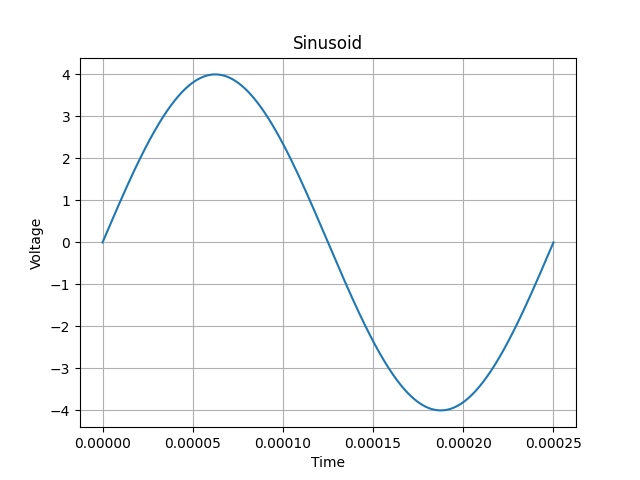
\includegraphics[width=0.7\textwidth]{figs/Figure_2.png}
		\caption*{(a) Plot of the sinusoid}
	\end{figure}
	
	\begin{figure}[htbp]
		\centering
		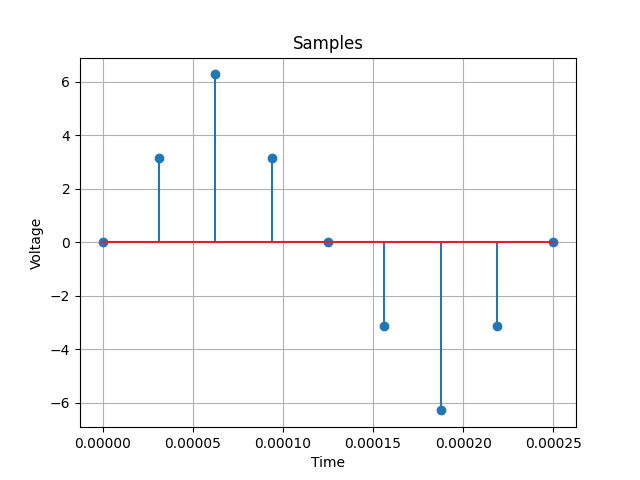
\includegraphics[width=0.7\textwidth]{figs/Figure_1.png}
		\caption*{(b) Plot of the samples with $\delta_{min}$}
	\end{figure}
\end{document}